


\noindent \textbf{Discrete memoryless channel (from last lecture)}
\begin{itemize}
\item For a DMC with ``m" inputs and ``n" outputs, the input X consists of input symbols $x_1, x_2, \ldots x_m$.
\item The probabilities of these source symbols $P(x_i)$ are assumed to be known.
\item The output Y consists of output symbols $\{y_1,y_2,\ldots, y_n \}$
\item Each possible input-to-output path is indicated along with a conditional probability $P(y_j|x_i)$, where $P(y_j|x_i)$  is the conditional probability of
obtaining output $y_j$ given that the input is $x_i$. \item $P(y_j|x_i)$ is called a \textbf{\emph{channel transition probability}}.
\end{itemize}

%\end{document}
%--------------------------------------------------------%
%--------------------------------------------------------%

\noindent \textbf{Discrete memoryless channel}
\vspace{-1cm}
\begin{itemize}
\item On the next slide, we present a binary DMC, with the channel transition probabilities indicated.
\item $P(y_1|x_1)$ = 0.9  and $P(y_2|x_1)$ = 0.1
\item $P(y_1|x_2)$ = 0.2  and $P(y_2|x_2)$ = 0.8
\end{itemize}


{
\noindent \textbf{Discrete Memoryless Channels}

\begin{center}
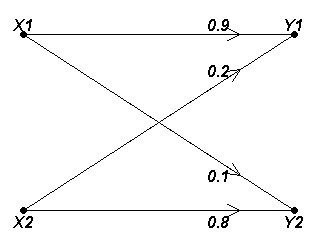
\includegraphics[scale=0.54]{10Bnet2}
\end{center}
}
%- Data Compression ( www.datacompression.com )


\noindent \textbf{Channel Matrix}

A channel is completely specified by the complete set of transition probabilities. Accordingly, a
channel is specified by the matrix of transition probabilities $[P(Y|X)]$, given by

\[  [P(Y|X)]  = \left[ \begin{array}{cccc}
P(y_1|x_1) & P(y_2|x_1) & \ldots & P(y_n|x_1) \\
P(y_1|x_2) & P(y_2|x_2) & \ldots & P(y_n|x_2) \\
\ldots & \ldots & \ldots & \ldots \\
P(y_1|x_m) & P(y_2|x_m) & \ldots & P(y_n|x_n) \\
\end{array} \right] \]


The matrix $[P(Y|X)]$ is called the \textbf{\emph{channel matrix}}.
%ZP(yylx;) : l lor all 1 (10.12)
 


\noindent \textbf{Channel Matrix}
\begin{itemize}
\item Since each input to the channel results in some
output, each row of the channel matrix must sum to unity (i.e. all rows must add up to 1. This condition is not necessary for columns).
\item For the binary DMC presented previously, the channel matrix is
\[  [P(Y|X)]  = \left[ \begin{array}{cc}
0.9 & 0.1  \\
0.2 & 0.8 \\
\end{array} \right] \]
\item (Remark: This is not the same as a binary symmetric channel (relevant to later material)
\end{itemize}




\noindent \textbf{Channel Matrix}
\begin{itemize}
\item The input probabilities $P(X)$ are represented by the row matrix
\[  [P(X)]  = \left[ \begin{array}{cccc}
P(x_1) & P(x_2) & \ldots & P(x_m) \\
\end{array} \right] \]
\item The output probabilities $P(Y)$ are represented by the row matrix
\[  [P(Y)]  = \left[ \begin{array}{cccc}
P(y_1) & P(y_2) & \ldots & P(y_n) \\
\end{array} \right] \]
\item We can compute $[P(Y)] $ by the following formula: $[P(Y)]  = [P(X)]\times [P(Y|X)]$
\item (Note: Be mindful of the dimensions of each matrix).
\end{itemize}



\noindent \textbf{Channel Matrix}
\begin{itemize}
\item Suppose for our Binary DMC that the input probabilities were given by $[P(X)] = [ 0.5\mbox{   }0.5]$.
\item Compute $[P(Y)]$, given the channel matrix given in previous slides.
\[  [P(Y)]  =  \left[ \begin{array}{cc}
0.5 & 0.5 \\
\end{array} \right] \times \left[ \begin{array}{cc}
0.9 & 0.1  \\
0.2 & 0.8 \\
\end{array} \right] \]

\item Solving
\[  [P(Y)]  =  \left[ \begin{array}{cc}
(0.5 \times 0.9)+(0.5 \times 0.2) & (0.5 \times 0.1)+(0.5 \times 0.8) \\
\end{array} \right]  \]

\item Simplifying \[  [P(Y)]  =  \left[ \begin{array}{cc}
0.55 & 0.45 \\
\end{array} \right]  \]
\end{itemize}




\noindent \textbf{Channel Matrix}
\begin{itemize}
\item Let $[P(X)]$ is presented as a diagonal matrix , i.e.

\[  [P(X)]_d  = \left[ \begin{array}{cccc}
P(x_1) &0 & \ldots & 0 \\
0 & P(x_2)& \ldots & 0 \\
\ldots & \ldots & \ldots & \ldots \\
0& 0 & \ldots & P(x_m) \\
\end{array} \right] \]
\item The \emph{\textbf{ joint probability matrix}} $[P(X,Y)]$can be computed as
$[P(X,Y)]  = [P(X)]_d\times [P(Y|X)]$
\end{itemize}



\noindent \textbf{Channel Matrix}
\begin{itemize}
\item For the Binary DMC described in the previous example, compute the joint probability matrix.
\item Diagonalize the input probabilities for $X$.
\[  [P(X)]_d  = \left[ \begin{array}{cc}
0.5 & 0.0  \\
0.0 & 0.5\\
\end{array} \right] \]

\item Simplifying
\[  [P(X,Y)]  =  \left[ \begin{array}{cc}
(0.5 \times 0.9)+(0 \times 0.2) & (0.5 \times 0.1)+(0 \times 0.8) \\
(0 \times 0.9)+(0.5 \times 0.2) & (0 \times 0.1)+(0.5 \times 0.8) \\
\end{array} \right]  \]


\item Solving
\[  [P(X,Y)]  =  \left[ \begin{array}{cc}
0.45 & 0.05 \\
0.1  & 0.4 \\
\end{array} \right]  \]
\end{itemize}

%---------------------------------------------------------------------------------------------------------------------------------------------------%

\noindent \textbf{Types of Channel}
\textbf{ 1. Lossless Channel:}\\
A channel described by a channel matrix with only one non-zero element in each column is called a lossless channel.


\[  [P(Y|X)]  =  \left[ \begin{array}{ccccc}
3/4 & 1/4 &0 & 0&0\\
0  & 0 &1/3 & 2/3& 0\\
0  & 0& 0&0 &1 \\
\end{array} \right]  \]
%(Drawn in overhead):\\ \bigskip

It can be shown that in the lossless channel, no source information is lost in transmission.

%---------------------------------------------------------------------------------------------------------------------------------------------------%

\noindent \textbf{Types of Channel}
\textbf{ 1. Lossless Channel:}\\

\begin{figure}
\centering
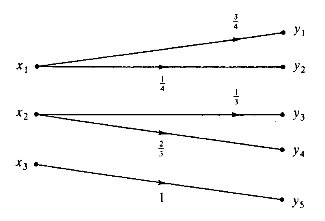
\includegraphics[width=0.7\linewidth]{./11Blossless}
\caption{}
\label{fig:11Blossless}
\end{figure}




%---------------------------------------------------------------------------------------------------------------------------------------------------%

\noindent \textbf{Types of Channel}
\textbf{2. Deterministic Channel:}\\
A channel described by a channel matrix with only one non-zero element in each row is called a deterministic channel.

\[  [P(Y|X)]  =  \left[ \begin{array}{ccc}
1   & 0 &0 \\
1  & 0 &0\\
0  & 1 &0\\
0  & 1& 0 \\
0  & 0& 1 \\
\end{array} \right]  \]
%(Drawn in overhead):\\ \bigskip
Note that since each row has only one non-zero element, this element must be 1. When a given source symbol is sent in a deterministic channel, it is clear which output symbol would be received.


%---------------------------------------------------------------------------------------------------------------------------------------------------%

\noindent \textbf{Types of Channel}
\textbf{2. Deterministic Channel:}\\
\begin{figure}
\centering
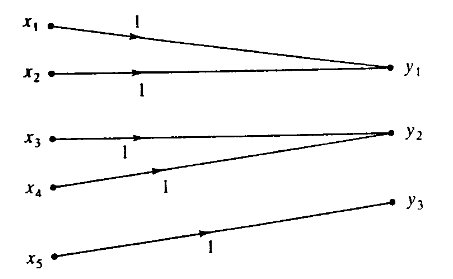
\includegraphics[width=0.7\linewidth]{./11Bdeterministic}
\caption{}
\label{fig:11Bdeterministic}
\end{figure}



%---------------------------------------------------------------------------------------------------------------------------------------------------%

\noindent \textbf{Types of Channel}
\textbf{3. Noiseless Channel:}\\
A channel is said to be \emph{\textbf{noiseless}} if it is both lossless and deterministic.
The channel matrix is the identity matrix: only one element in each row and each column, and each element is necessarily 1.
\[  [P(Y|X)]  = \left[ \begin{array}{cccc}
1 &0 & \ldots & 0 \\
0 & 1& \ldots & 0 \\
\ldots & \ldots & \ldots & \ldots \\
0& 0 & \ldots & 1 \\
\end{array} \right] \]
%(Drawn in overhead):\\ \bigskip
Note that the input and output alphabets have the same size , i.e. $m=n$.


\noindent \textbf{Types of Channel}
\textbf{3. Noiseless Channel:}\\
\begin{figure}
\centering
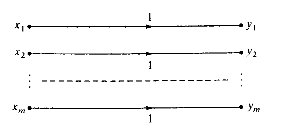
\includegraphics[width=0.7\linewidth]{./11BNoiseless}
\caption{}
\label{fig:11BNoiseless}
\end{figure}


%----------------------------------------------------------------------------------------------------------------------------------------------------%

\noindent \textbf{Types of Channel}
\textbf{4. Binary Symmetric Channel:}\\
The binary symmetric channel is defined by the following channel diagram (next slide) and the channel matrix is given by

\[  [P(Y|X)]  = \left[ \begin{array}{cc}
1-p & p  \\
p & 1-p\\
\end{array} \right] \]
The channel has two inputs and two outputs $(x_1=0,x_2=1)$ and two outputs $(x_1=0,x_2=1)$. The channel is symmetric because the probability of receiving a 1 if a 0 is sent is the same as the probability of receiving a 0 if a 1 was sent. This common probability is denoted $p$.


{
\noindent \textbf{Binary Symmetric Channels}

\begin{center}
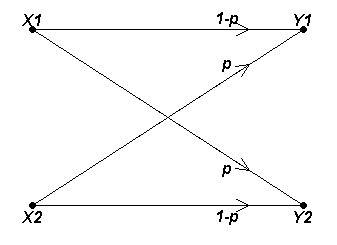
\includegraphics[scale=0.54]{11aBSC}
\end{center}
}




%----------------------------------------------------------------------------------%
{
\noindent \textbf{Entropy: some remarks}
\begin{itemize}
\item recall: Entropy is the uncertainty of a single random variable. \item We can define \textbf{\emph{conditional entropy }}$H(X|Y)$, which is the entropy of a random variable
conditional on the knowledge of another random variable. \item The reduction in uncertainty due to another random variable is called the \textbf{\emph{mutual information}}.
\end{itemize}
}


\noindent \textbf{Code efficiency and Code redundancy}
% Pg 253/254
The parameter $L$ represents the average number of bits per source symbol used in the source coding process.
The code efficiency is defined as \[\nu = {L_{min} \over L} \]where $L_{min}$ is the minimum possiblve value of $L$. When $\nu$ approaches unity, the codes is said to be efficient.
The code redundancy $\gamma$ is defined as $\gamma = 1- \nu$.



%---------------------------------------------------------------------------------------------------------------------------------------%

%page 254
\noindent \textbf{Source Coding Theorem}
The source coding theorem states that for zi DMS X with entropy $H(X)$, the average code word length $L$ per symbol is bounded as
L 2 H(X) (10.52)

and further, L can bc made as close to H(X) as dcsircd for some suitably chosen code.
Thus, with$ L_{min} \geq H(X)$.

The code efficiency can be rewritten as
\[\nu = {H(X) \over L} \]


%-----------------------------------------------------------------------------------------------%
 % ULCIS
\noindent \textbf{Self Information}Self-information
This is defined by the following mathematical formula:$I(A) = −logb P(A)$

The self-information of an event measures the amount of one's surprise
evoked by the event. The negative logarithm $−logb P(A)$ can also be written as \[
log_b  {1 \over P(A)} \]
Note that log(1) = 0, and that $| − log(P(A))|$ increases as P(A) decreases
from 1 to 0. This supports our intuition from daily experience. For example,
a low-probability event tends to cause more ``surprise".



%-------------------------------------------------------------------------------------------%
{
\noindent \textbf{Example}
For a simple example, we will take a short phrase and derive our probabilities from a frequency count of letters within that phrase. The resulting encoding should be good for compressing this phrase, but of course will be inappropriate for other phrases with a different letter distribution.

"All you base are belong to us"
}


%----------------------------------------------------------------------------------%
{
\noindent \textbf{Entropy}
\begin{itemize}
\item Entropy is the uncertainty of a single random variable. \item We can define \textbf{\emph{conditional entropy }}$H(X|Y)$, which is the entropy of a random variable
conditional on the knowledge of another random variable. \item The reduction in uncertainty due to another random variable is called the \textbf{\emph{mutual information}}.
\end{itemize}
}
%----------------------------------------------------------------------------------%



%----------------------------------------------------------------------------------%
{
\begin{description}[Second Item]
\item[First Item] Description of first item
\item[Second Item] Description of second item
\item[Third Item] Description of third item
\item[Forth Item] Description of forth item
\end{description}

}


{
\noindent \textbf{What is Information?}
\begin{itemize} \item Once we agree to define the information of an event ain terms of P(a), the properties (2) and (3) will be satisfied if the information in ais defined as
\[ I(a) = -log P(a)\]

\item Remark : The base of the logarithm depends on the unit of information to be used.
\end{itemize}
}



%-------------------------------------------------------------------------------------------%
{
Ambiguity occurs if there is any path to some symbol whose label is a prefix of the label of a path to some other symbol. In the Huffman tree, every symbol is a \textbf{\emph{leaf}}. Thus it is impossible for the label of a path to a leaf to be a prefix of any other path label, and so the mapping defined by Huffman coding has an inverse and decoding is possible.
}
%-------------------------------------------------------------------------------------------%
{
\noindent \textbf{Example}
For a simple example, we will take a short phrase and derive our probabilities from a frequency count of letters within that phrase. The resulting encoding should be good for compressing this phrase, but of course will be inappropriate for other phrases with a different letter distribution.

"All you base are belong to us"
}




